\documentclass[letterpaper,12pt]{article}
\usepackage{fullpage}
\usepackage{amsmath}
\usepackage{graphicx}
\usepackage{epsfig}

% This last command gives the possibility of variable line spacing.
\renewcommand{\baselinestretch}{1.1}
\newcommand{\bqu}{\begin{quote} \it}
\newcommand{\equ}{\end{quote}}
\newcommand{\beqn}{\begin{eqnarray}}
\newcommand{\eeqn}{\end{eqnarray}}
\newcommand{\nonu}{\nonumber \\}
\newcommand{\br}{\langle}
\newcommand{\ke}{\rangle}
\def\f#1#2{\frac{#1}{#2}}

\def\ni{\noindent}
\def\J{{\rm\,J}}
\def\W{{\rm\,W}}
\def\s{{\rm\,s}}
\def\erg{{\rm\,erg}}
\def\cm{{\rm\,cm}}
\def\m{{\rm\,m}}
\def\km{{\rm\,km}}
\def\kg{{\rm\,kg}}
\def\mm{{\rm\,mm}}
\def\gm{{\rm\,g}}
\def\g{{\rm\,g}}
\def\d{\rm\,d}
\def\h{\rm\,h}
\def\mum{\,\mu{\rm m}}
\def\K{{\rm\,K}}
\def\yr{{\rm\,yr}}
\def\Hz{{\rm\,Hz}}
\def\days{{\rm\,days}}
\def\cals{{\rm\,cals}}
\def\mole{{\rm\,mole}}
\def\gal{{\rm\,gal}}
\def\calo{\,{\rm calorie}}
\def\dyne{\,{\rm dyne}}
\def\s{\,{\rm s}}
\def\at{\, {\rm atmosphere}}
\def\J{\,{\rm joule}}
\def\pomega{\tilde{\omega}}
\def\vs{\vspace{0.1in}}
\def\n{\vspace{0.1in} \ni }

\begin{document}

Max Genecov

\begin{center}
\Large Stellar Populations Homework 2 
\end{center}

\normalsize
\section{Wikipedia Is Sloppy}

The problem with the Wikipedia page is that it reports Salpeter's initial assessment of the slope of the IMF is 2.35. In fact, it is -1.35. This is due to the difference in the log scales classically used. In Scalo 1986 parlance, he reported $-\Gamma(m)$ when Wikipedia says he reported $-\gamma(m)$.

\section{Playing with a Model IMF}

All my work on this problem is in the jupyter notebook, but my overall problem is trying to reconcile the difference between the normalization of the probability and the normalization of the histograms themselves. I understand that, in an ideal sense, I shouldn't be using histograms and fitting power laws to them, but that is all I can do to approximate a mass function. I could recover the power law $\alpha$, but not $M_{max} $. I would appreciate it if you could explain in class how to work out this normalization problem or how to work around it.

\section{Redoing Salpeter}

Once again all the relevant work is on the web, but I will put my lingering questions here. I am fitting the data in log-space already, so it seems likely enough to just fit a line to this logged data and then work backwards to discover a power law in linear space. Everything looks good on this front except for the fact that the constant is confusing. I can recover Salpeter's constant of 0.03 if I recognize that I should log this constant as well and then subtract 1 from it since 

$$ \xi = 0.03 (\frac{M}{M_{\odot}})^{-1.35} \Rightarrow \ln \ \xi = \ln (0.03)+1.35 -1.35(\ln (M))$$

And so my constant of 9.94 gives the somewhat magical equation $\ln (9.94) \approx -(\ln(0.03) + 1.35) $. If I were to flip the direction of integration and log my values in such a way, I would end up with $\xi_0 = .026 \pm .0015$, which I guess is what I'll go with.

\section{Chabrier and Kroupa}

Nothing much to say here other than I'm a bit surprised that the values of alpha don't line up more precisely. All the work is in the notebook.

Also, when ever I think of Pavel Kroupa, I think of the Koopa Troopa enemy from Super Mario, so now you at least know what I'm thinking about when doing this homework.

\section{Python FSPS}

Finally, I wasn't able to get FSPS to work on the notebook, so I at least included my console commands in the notebook, even though they won't run from there.

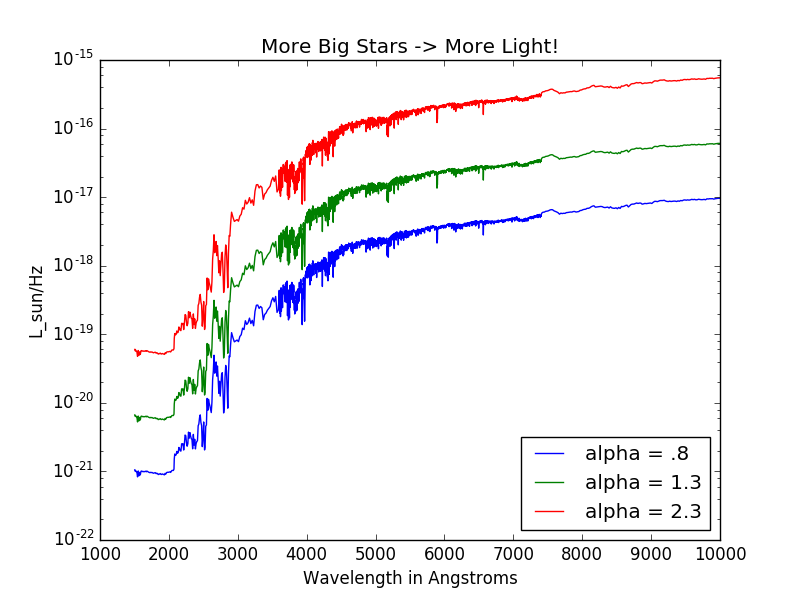
\includegraphics[width = 5in]{threealphas}

Unsurprisingly, this first graphs shows that, if one has a shallower power law, there will be higher mass stars initially and at ten million years after star formation, and there will therefore these big stars will yield more light.

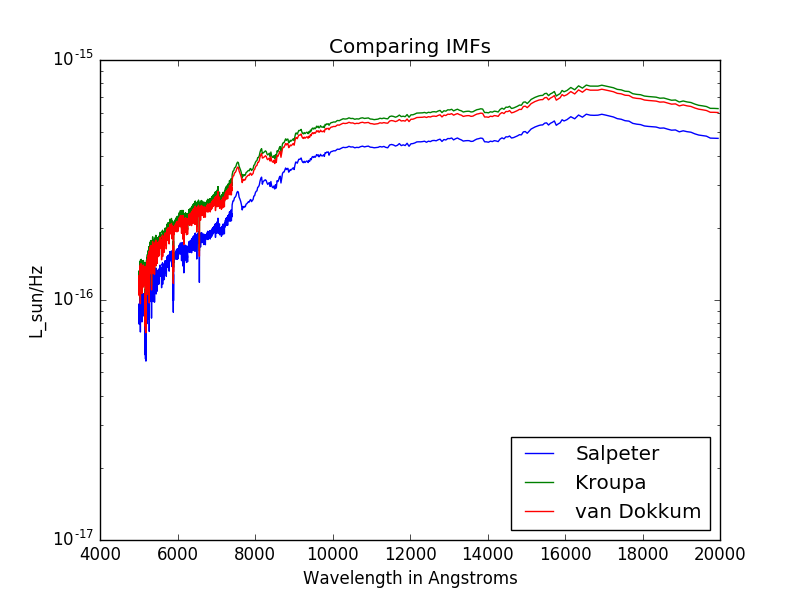
\includegraphics[width = 5in]{ComparingIMFs}

Here we are probing much lower mass stars, both because of the range of the spectrum and because this population is ten billion years old. The Salpeter IMF, since it is so steep, has fewer luminous stars. In other words, its low mass is even lower than what we're dealing with here.

The Kroupa and Van Dokkum IMFs look quite similar. The Kroupa power law likely has its break at higher masses than those whose light we see here, so its normalization is higher, and so we see more higher mass stars here than we do in the Salpeter IMF. As for the Van Dokkum, it is a bottom-heavy IMF as well that implies a steeper power law at very low masses than Salpeter. I therefore don't quite understand why it is so close to the Kroupa value!


\end{document}
